\section{Resultados}
En esta sección se presentan los resultados experimentales obtenidos del algoritmo Regret Matching, el cual fue probado con los juegos descritos anteriormente. Cada procedimiento fue probado con cada juego $10$ veces, cada corrida fue finalizada cuando el regret máximo era menor a $0.005$.

Para todos los juegos, con excepción del juego Coronel Blotto, se presenta una tabla con las estrategias obtenidas en la última corrida de cada uno de los procedimientos, así como la estrategia correspondiente al equilibrio de Nash. En estas tablas, también se añade el \textit{peor caso} para cada jugador, esto es, la utilidad esperada del jugador si su oponente juega con una estrategia que sea mejor respuesta a la estrategia empleada, y del teorema \ref{theo:mejor-respuesta}, se obtiene que existe una estrategia que es mejor respuesta cuyo soporte tiene un sólo elemento. Por lo que el menor valor posible para la utilidad esperada del jugador $i$ al utilizar la estrategia $\sigma_i$ viene dada por:
\begin{alignat}{1}
min_{s_{-i} \in S_{-i}} u_i(\sigma_i, s_{-i})
\end{alignat}
Donde $u_i(\sigma_i, s_{-i})$ representa la utilidad esperada del jugador $i$, cuando juega con la estrategia mixta $\sigma_i$ y su oponente juega con la estrategia pura $s_i$. Estos valores son represetados con las variables $v_1$ y $v_2$ en cada una de las tablas con las estrategias respectivas.

Por otra parte, para todos los juegos se presenta una tabla que indica el tiempo de cada corrida ($T$), el número de iteraciones para alcanzar la cota deseada ($I$) y el tiempo promedio de cada iteración en cada una de las corridas ($T/I$), así como el promedio del tiempo y del número de iteraciones para cada procedimiento. Además, también se muestran las gráficas del regret por iteraciones, para observar su convergencia. Estas gráficas se presentan en una escala logarítmica en el eje $x$ para apreciar mejor los resultados.

\subsection{Matching Pennies}
En este juego ambos jugadores pueden garantizar una utilidad esperada de $0$, sin importar la estrategia utilizada por su oponente, que se obtiene al jugar con una estrategia de $0.5$ para ambas acciones posibles de cada jugador. Las estrategias obtenidas no corresponden al equilibrio de Nash exacto, sin embargo, garantizan una utilidad cercana a $0$ en todos los casos, siendo la más baja igual a $-0.01$, como se muestra en la Tabla \ref{tab:estrategias-matching-pennies}.

\begin{table}[ht]
    \centering
    \begin{tabular}{c|c|c|c|c}
        & E.N. & A & B & C \\ \hline
        $\sigma_1$   & $(0.500, 0.500)$ & $( 0.505, 0.495)$ & $( 0.504, 0.496)$ & $(0.500,  0.500)$ \\
        $\sigma_2$   & $(0.500, 0.500)$ & $( 0.500, 0.500)$ & $( 0.500, 0.500)$ & $(0.505,  0.495)$ \\ \hline
        $(v_1, v_2)$ & $(0.000, 0.000)$ & $(-0.010, 0.000)$ & $(-0.008, 0.000)$ & $(0.000, -0.010)$ \\ \hline
    \end{tabular}
    \caption{Estrategias obtenidas del juego Matching Pennies}
    \label{tab:estrategias-matching-pennies}
\end{table}


La Tabla \ref{tab:resultados-matching-pennies} muetra los resultados obtenidos relacionados al tiempo y número de iteraciones de los prodemientos. El procedimiento A, regret condicional, tuvo una duración promedio de $85.314$ segundos, con un número promedio de iteraciones de $5609971.5$, obteniendo un promedio de $1.52 {\times} 10^{-5}$ segundos por iteración. Con el procedimiento B, que utiliza un vector invariante de probabilidad, se obtuvo un tiempo, número de iteraciones y tiempo por iteración promedios de $3.503$ segundos, $30277.9$ iteraciones y $1.16 {\times} 10^{-4}$ segundos por iteración, respectivamente. Por último, el procedimiento C, regret incondicional, se obtuvo un tiempo promedio de $0.217$, el número de iteraciones promedio fue de $14806.8$, obteniendo un promedio de $1.47 {\times} 10^{-5}$ segundos por iteración. 

\begin{table}[ht]
\scriptsize
    \centering
    \begin{tabular}{r r r | r r r | r r r}
    \multicolumn{3}{c}{A} & \multicolumn{3}{c}{B} & \multicolumn{3}{c}{C} \\ \hline
    $T$ & $I$ & $T/I$ & $T$ & $I$ & $T/I$ & $T$ & $I$ & $T/I$ \\  \hline
    $375.559$ & $24597798$ & $1.53 {\times} 10 ^{-5}$ & $10.616$ & $91683$ & $1.16 {\times} 10 ^{-4}$ & $0.155$ & $10553$ & $1.47 {\times} 10 ^{-5}$ \\
    $20.442$ & $1349708$ & $1.51 {\times} 10 ^{-5}$ & $2.407$ & $20797$ & $1.16 {\times} 10 ^{-4}$ & $0.173$ & $11847$ & $1.46 {\times} 10 ^{-5}$ \\
    $22.030$ & $1455882$ & $1.51 {\times} 10 ^{-5}$ & $1.465$ & $12674$ & $1.16 {\times} 10 ^{-4}$ & $0.048$ & $3302$ & $1.46 {\times} 10 ^{-5}$ \\
    $39.273$ & $2591911$ & $1.52 {\times} 10 ^{-5}$ & $0.529$ & $4576$ & $1.16 {\times} 10 ^{-4}$ & $0.047$ & $3201$ & $1.46 {\times} 10 ^{-5}$ \\
    $141.703$ & $9307528$ & $1.52 {\times} 10 ^{-5}$ & $9.403$ & $81270$ & $1.16 {\times} 10 ^{-4}$ & $0.373$ & $25370$ & $1.47 {\times} 10 ^{-5}$ \\
    $73.271$ & $4837112$ & $1.51 {\times} 10 ^{-5}$ & $1.453$ & $12570$ & $1.16 {\times} 10 ^{-4}$ & $0.453$ & $30866$ & $1.47 {\times} 10 ^{-5}$ \\
    $21.917$ & $1451479$ & $1.51 {\times} 10 ^{-5}$ & $0.692$ & $6017$ & $1.15 {\times} 10 ^{-4}$ & $0.147$ & $10040$ & $1.47 {\times} 10 ^{-5}$ \\
    $10.238$ & $678965$ & $1.51 {\times} 10 ^{-5}$ & $4.205$ & $36371$ & $1.16 {\times} 10 ^{-4}$ & $0.263$ & $17963$ & $1.46 {\times} 10 ^{-5}$ \\
    $61.776$ & $4087347$ & $1.51 {\times} 10 ^{-5}$ & $2.201$ & $19018$ & $1.16 {\times} 10 ^{-4}$ & $0.193$ & $13176$ & $1.47 {\times} 10 ^{-5}$ \\
    $86.932$ & $5741985$ & $1.51 {\times} 10 ^{-5}$ & $2.057$ & $17803$ & $1.16 {\times} 10 ^{-4}$ & $0.319$ & $21750$ & $1.47 {\times} 10 ^{-5}$ \\ \hline
    $85.314$ & $5609971.5$ & $1.52 {\times} 10 ^{-5}$ & $3.503$ & $30277.9$ & $1.16 {\times} 10 ^{-4}$ & $0.217$ & $14806.8$ & $1.47 {\times} 10 ^{-5}$ \\ \hline
    \end{tabular}
    \caption{Resultados del juego Matching Pennies}
    \label{tab:resultados-matching-pennies}
\end{table}

La Figura \ref{fig:regret-matching-pennies} muestra el regret incondicional con respecto al tiempo de la última corrida, para los $3$ procedimientos.

\begin{figure}[ht]
\caption{Gráficas del regret con respecto al número de iteraciones del juego Matching Pennies}
\label{fig:regret-matching-pennies}
\centering
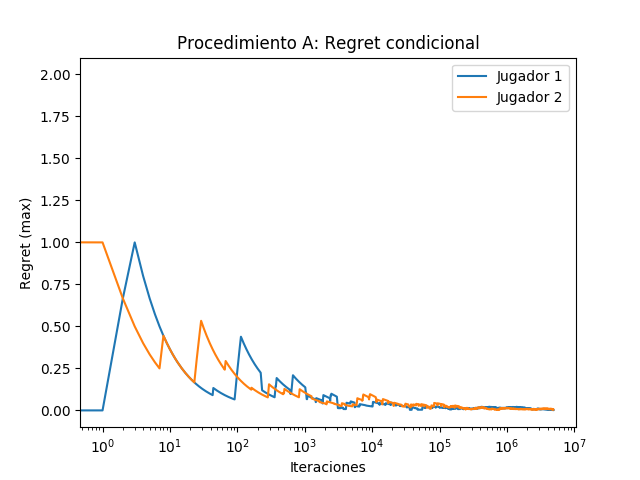
\includegraphics[width=0.327\textwidth]{graficas/matching-pennies/procedimiento-A.png}
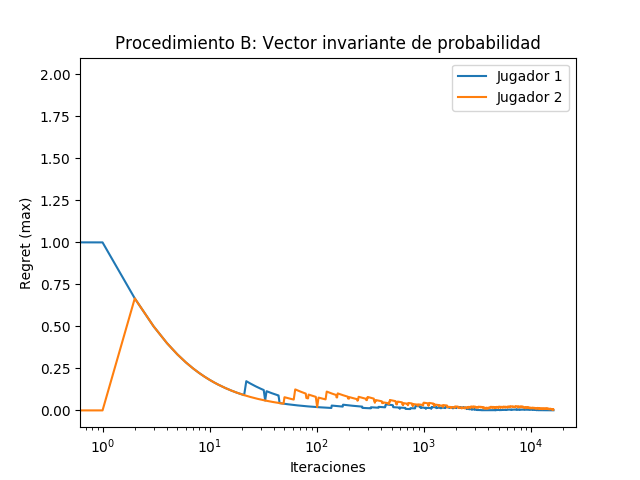
\includegraphics[width=0.327\textwidth]{graficas/matching-pennies/procedimiento-B.png}
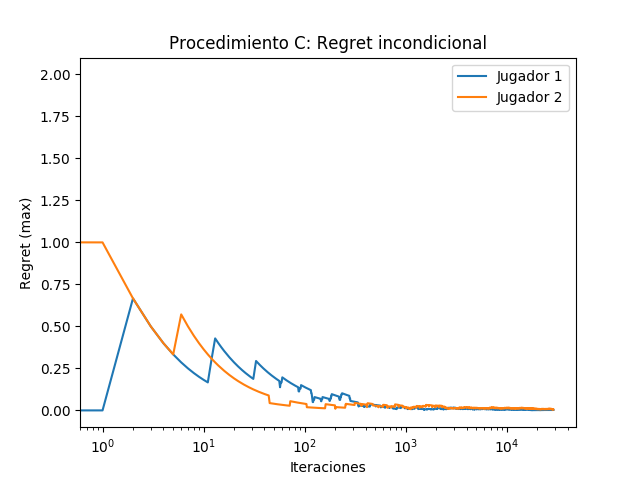
\includegraphics[width=0.327\textwidth]{graficas/matching-pennies/procedimiento-C.png}
\end{figure}

\subsection{Piedra, Papel o Tijeras}

En este juego, al igual que en el anterior, ambos jugadores pueden garantizar una utilidad esperada de $0$ sin importar la estrategia utilizada por su oponente, que se obtiene al elegir las opciones con igual probabilidad. No todas las estrategias obtenidas corresponden al equilibrio de Nash exacto, sin embargo, garantizan una utilidad cercana a $0$ en todos los casos, siendo la más baja igual a $-0.008$, como se muestra en la Tabla \ref{tab:estrategias-RPS}.

\begin{table}[ht]
    \centering
    \scriptsize
    \begin{tabular}{c|c|c|c|c}
        & E.N. & A & B & C \\ \hline
        $\sigma_1$ &  $(0.333, 0.333, 0.333)$ & $(0.330, 0.333, 0.337)$ & $(0.333, 0.333, 0.333)$ & $(0.333, 0.334, 0.333)$ \\
        $\sigma_2$ &  $(0.333, 0.333, 0.333)$ & $(0.335, 0.330, 0.335)$ & $(0.333, 0.333, 0.333)$ & $(0.335, 0.338, 0.327)$ \\ \hline
        $(v_1, v_2)$ & $(0.000, 0.000)$ & $(-0.004, -0.005)$ & $(0.000, 0.000)$ & $(-0.001, -0.008)$ \\ \hline
    \end{tabular}
    \caption{Estrategias obtenidas del juego Piedra, Papel o Tijeras}
    \label{tab:estrategias-RPS}
\end{table}

La Tabla \ref{tab:resultados-RPS} muetra los resultados obtenidos relacionados al tiempo y número de iteraciones de los prodemientos. El procedimiento A, regret condicional, tuvo una duración promedio de $56.231$ segundos, con un número promedio de iteraciones de $3671952.7$, obteniendo un promedio de $1.53 {\times} 10^{-5}$ segundos por iteración. Con el procedimiento B, que utiliza un vector invariante de probabilidad, se obtuvo un tiempo, número de iteraciones y tiempo por iteración promedios de $1.732$ segundos, $1007$ iteraciones y $1.73 {\times} 10^{-4}$ segundos por iteración, respectivamente. Por último, el procedimiento C, regret incondicional, se obtuvo un tiempo promedio de $0.449$, el número de iteraciones promedio fue de $30293.6$, obteniendo un promedio de $1.48 {\times} 10^{-5}$ segundos por iteración.

\begin{table}[ht]
    \scriptsize
    \centering
    \begin{tabular}{r r r | r r r | r r r}
    \multicolumn{3}{c}{A} & \multicolumn{3}{c}{B} & \multicolumn{3}{c}{C} \\ \hline
    $T$ & $I$ & $T/I$ & $T$ & $I$ & $T/I$ & $T$ & $I$ & $T/I$ \\  \hline
    $64.6323$ & $4222223$ & $1.53 {\times} 10 ^{-5}$ & $0.000448982$ & $3$ & $1.50 {\times} 10 ^{-4}$ & $0.913989$ & $61642$ & $1.48 {\times} 10 ^{-5}$ \\
    $23.6302$ & $1549016$ & $1.53 {\times} 10 ^{-5}$ & $3.53961$ & $20371$ & $1.74 {\times} 10 ^{-4}$ & $0.16622$ & $11228$ & $1.48 {\times} 10 ^{-5}$ \\
    $99.8796$ & $6513228$ & $1.53 {\times} 10 ^{-5}$ & $0.774109$ & $4494$ & $1.72 {\times} 10 ^{-4}$ & $0.722437$ & $48801$ & $1.48 {\times} 10 ^{-5}$ \\
    $79.7865$ & $5192787$ & $1.54 {\times} 10 ^{-5}$ & $0.684216$ & $3951$ & $1.73 {\times} 10 ^{-4}$ & $0.314035$ & $21037$ & $1.49 {\times} 10 ^{-5}$ \\
    $23.5387$ & $1544402$ & $1.52 {\times} 10 ^{-5}$ & $0.000385862$ & $3$ & $1.29 {\times} 10 ^{-4}$ & $0.394145$ & $26588$ & $1.48 {\times} 10 ^{-5}$ \\
    $15.1729$ & $998763$ & $1.52 {\times} 10 ^{-5}$ & $0.000436849$ & $3$ & $1.46 {\times} 10 ^{-4}$ & $0.362224$ & $24441$ & $1.48 {\times} 10 ^{-5}$ \\
    $49.3657$ & $3234372$ & $1.53 {\times} 10 ^{-5}$ & $6.0129$ & $34711$ & $1.73 {\times} 10 ^{-4}$ & $0.249781$ & $16869$ & $1.48 {\times} 10 ^{-5}$ \\
    $37.4907$ & $2448062$ & $1.53 {\times} 10 ^{-5}$ & $2.32126$ & $13362$ & $1.74 {\times} 10 ^{-4}$ & $0.620189$ & $41841$ & $1.48 {\times} 10 ^{-5}$ \\
    $124.844$ & $8144322$ & $1.53 {\times} 10 ^{-5}$ & $3.98568$ & $23166$ & $1.72 {\times} 10 ^{-4}$ & $0.369477$ & $24980$ & $1.48 {\times} 10 ^{-5}$ \\
    $43.9675$ & $2872352$ & $1.53 {\times} 10 ^{-5}$ & $0.00085012$ & $6$ & $1.42 {\times} 10 ^{-4}$ & $0.378752$ & $25509$ & $1.48 {\times} 10 ^{-5}$ \\ \hline
    $56.231$ & $3671952.7$ & $1.53 {\times} 10 ^{-5}$ & $1.732$ & $10007$ & $1.73 {\times} 10 ^{-4}$ & $0.449$ & $30293.6$ & $1.48 {\times} 10 ^{-5}$ \\\hline
    \end{tabular}
    \caption{Resultados del juego Piedra, Papel o Tijeras}
    \label{tab:resultados-RPS}
\end{table}

La Figura \ref{fig:regret-RPS} muestra el regret incondicional con respecto al tiempo de la última corrida para los procedimientos A, B y C.

\begin{figure}[ht]
\caption{Gráficas del regret con respecto al número de iteraciones del juego Piedra, Papel o Tijera}
\label{fig:regret-RPS}
\centering
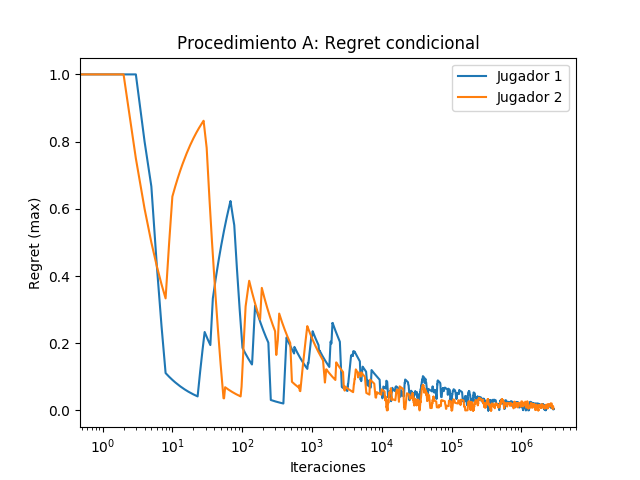
\includegraphics[width=0.327\textwidth]{graficas/RPS/procedimiento-A.png}
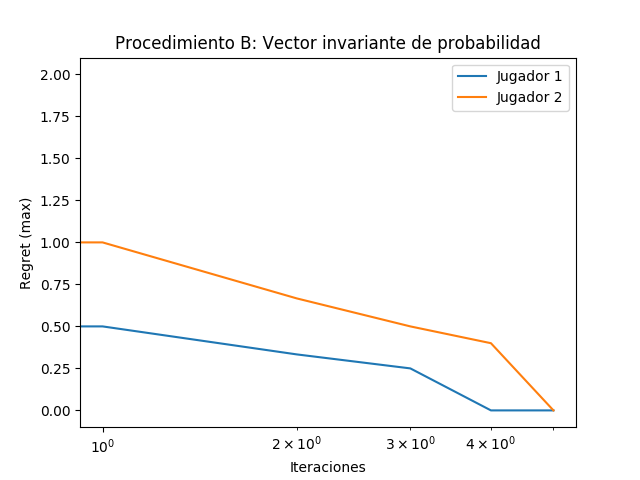
\includegraphics[width=0.327\textwidth]{graficas/RPS/procedimiento-B.png}
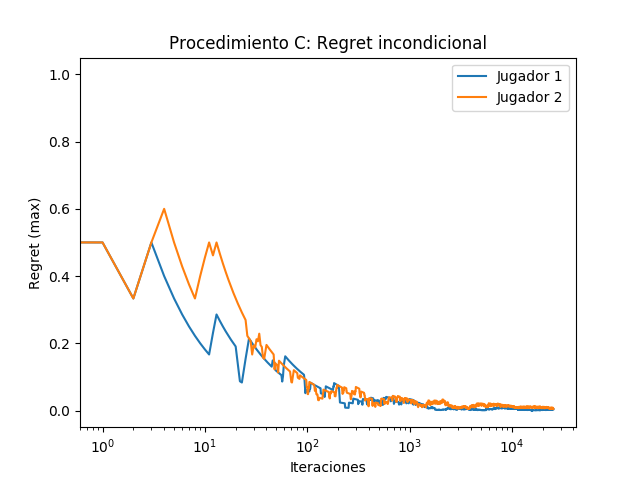
\includegraphics[width=0.327\textwidth]{graficas/RPS/procedimiento-C.png}
\end{figure}

\subsection{Dominó}

En este juego, el primer jugador puede garantizar una ganancia esperada de, al menos $1/3$, por lo que el segundo jugador puede garantizar no perder más de $1/3$. A diferencia de los juegos anteriores, la matriz de pagos de este juegos no es simétrica y el primer jugador tiene ventaja sobre el segundo. Además, este juego no tiene un equilibrio de Nas único. En la Tabla \ref{tab:estrategias-RPS} se observa que las estrategias obtenidas para el primer jugador le permiten obtener una ganancia esperada de $0.330$, $0.326$ y $0.329$, respectivamente para los procedimientos A, B y C. Todos estos valores son menores que $1/3$, pero con una diferencia menor que $0.01$. Por otra parte el segundo jugador puede garantizar un valor esperado no menor que $-0.338$, $-0.335$, $-0.335$.

\begin{table}[ht]
    \centering
    \begin{tabular}{c c|c|r}
        & & Estrategias & $v_1 / v_2$\\
        \hline
        \multirow{2}{*}{E.N.}
        & $\sigma_1$ & $(0.333, 0.333, 0.000, 0.000, 0.000, 0.000, 0.333)$ & $0.333$ \\
        & $\sigma_2$ & $(0.333, 0.000, 0.333, 0.000, 0.333, 0.000)$ &  $-0.333$\\
        \hline
        \multirow{2}{*}{A}
        & $\sigma_1$ & $(0.149, 0.152, 0.115, 0.114, 0.181, 0.069, 0.220)$ & $0.330$ \\
        & $\sigma_2$ & $(0.187, 0.148, 0.186, 0.147, 0.186, 0.147)$ & $-0.338$\\
        \hline
        \multirow{2}{*}{B}
        & $\sigma_1$ & $(0.143, 0.145, 0.138, 0.136, 0.192, 0.050, 0.196)$ & $0.326$ \\
        & $\sigma_2$ & $(0.167, 0.165, 0.168, 0.163, 0.167, 0.168)$ & $-0.335$\\
        \hline
        \multirow{2}{*}{C}
        & $\sigma_1$ & $(0.128, 0.130, 0.135, 0.134, 0.202, 0.071, 0.201)$ & $0.329$ \\
        & $\sigma_2$ & $(0.158, 0.177, 0.157, 0.175, 0.158, 0.176)$ & $-0.335$\\
        \hline
    \end{tabular}
    \caption{Estrategias obtenidas del juego Dominó}
    \label{tab:estrategias-domino}
\end{table}

La Tabla \ref{tab:resultados-domino} muetra los resultados obtenidos relacionados al tiempo y número de iteraciones de los prodemientos de este juego. El procedimiento A, regret condicional, tuvo una duración promedio de $1520.421$ segundos, con un número promedio de iteraciones de $91116271.5$, obteniendo un promedio de $1.67 {\times} 10^{-5}$ segundos por iteración. Con el procedimiento B, que utiliza un vector invariante de probabilidad, se obtuvo un tiempo, número de iteraciones y tiempo por iteración promedios de $28.381$ segundos, $63267.8$ iteraciones y $4.49 {\times} 10^{-4}$ segundos por iteración, respectivamente. Por último, el procedimiento C, regret incondicional, se obtuvo un tiempo promedio de $1.510098$, el número de iteraciones promedio fue de $95233.3$, obteniendo un promedio de $1.59 {\times} 10^{-5}$ segundos por iteración. 

\begin{table}[ht]
   \scriptsize
    \centering
    \begin{tabular}{r r r | r r r | r r r}
    \multicolumn{3}{c}{A} & \multicolumn{3}{c}{B} & \multicolumn{3}{c}{C} \\ \hline
    $T$ & $I$ & $T/I$ & $T$ & $I$ & $T/I$ & $T$ & $I$ & $T/I$ \\  \hline
    $740.447$ & $44412293$ & $1.67 {\times} 10 ^{-5}$ & $23.2266$ & $51679$ & $4.49 {\times} 10 ^{-4}$ & $1.41241$ & $89150$ & $1.58 {\times} 10 ^{-5}$ \\
    $1153.83$ & $69255567$ & $1.67 {\times} 10 ^{-5}$ & $33.3787$ & $74447$ & $4.48 {\times} 10 ^{-4}$ & $1.84509$ & $116261$ & $1.59 {\times} 10 ^{-5}$ \\
    $1344.98$ & $80595152$ & $1.67 {\times} 10 ^{-5}$ & $70.0653$ & $156038$ & $4.49 {\times} 10 ^{-4}$ & $2.13461$ & $134489$ & $1.59 {\times} 10 ^{-5}$ \\
    $2678.05$ & $160284767$ & $1.67 {\times} 10 ^{-5}$ & $23.2227$ & $51886$ & $4.48 {\times} 10 ^{-4}$ & $0.76709$ & $48213$ & $1.59 {\times} 10 ^{-5}$ \\
    $1091.08$ & $65511893$ & $1.67 {\times} 10 ^{-5}$ & $26.4452$ & $59056$ & $4.48 {\times} 10 ^{-4}$ & $0.334749$ & $21221$ & $1.58 {\times} 10 ^{-5}$ \\
    $365.475$ & $22030226$ & $1.66 {\times} 10 ^{-5}$ & $19.1969$ & $42825$ & $4.48 {\times} 10 ^{-4}$ & $1.98904$ & $125803$ & $1.58 {\times} 10 ^{-5}$ \\
    $2096.08$ & $125780618$ & $1.67 {\times} 10 ^{-5}$ & $14.4957$ & $32291$ & $4.49 {\times} 10 ^{-4}$ & $1.33082$ & $83575$ & $1.59 {\times} 10 ^{-5}$ \\
    $2835.32$ & $169464746$ & $1.67 {\times} 10 ^{-5}$ & $24.0569$ & $53610$ & $4.49 {\times} 10 ^{-4}$ & $2.35906$ & $148921$ & $1.58 {\times} 10 ^{-5}$ \\
    $1765.15$ & $105855204$ & $1.67 {\times} 10 ^{-5}$ & $27.2148$ & $60743$ & $4.48 {\times} 10 ^{-4}$ & $0.626211$ & $38952$ & $1.61 {\times} 10 ^{-5}$ \\
    $1133.8$ & $67972249$ & $1.67 {\times} 10 ^{-5}$ & $22.5033$ & $50103$ & $4.49 {\times} 10 ^{-4}$ & $2.3019$ & $145748$ & $1.58 {\times} 10 ^{-5}$ \\\hline
    $1520.421$ & $91116271.5$ & $1.67 {\times} 10 ^{-5}$ & $28.381$ & $63267.8$ & $4.49 {\times} 10 ^{-4}$ & $1.510098$ & $95233.3$ & $1.59 {\times} 10 ^{-5}$ \\ \hline
    \end{tabular}
    \caption{Resultados del juego Dominó}
    \label{tab:resultados-domino}
\end{table}

La Figura \ref{fig:regret-domino} muestra el regret incondicional con respecto al tiempo de la última corrida, para los procedimientos B y C.

\begin{figure}[ht]
\caption{Gráficas del regret con respecto al número de iteraciones del juego Dominó}
\label{fig:regret-domino}
\centering
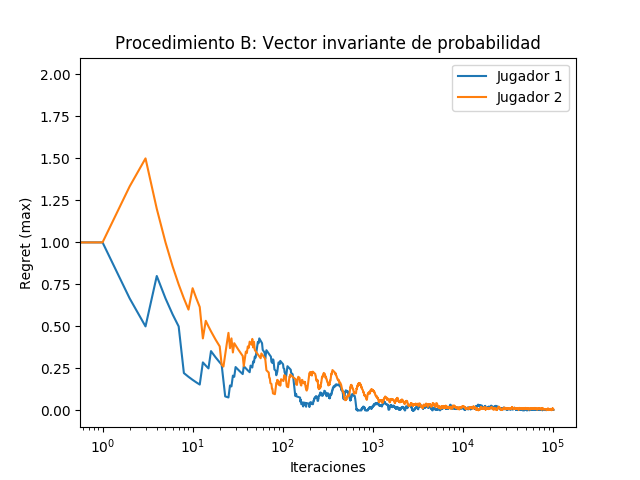
\includegraphics[width=0.4\textwidth]{graficas/domino/procedimiento-B.png}
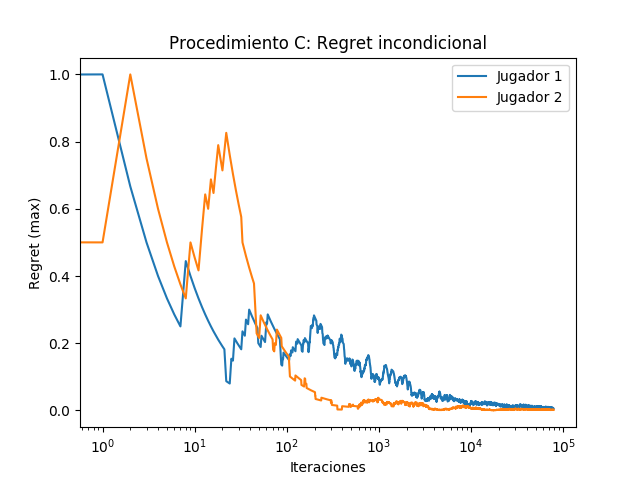
\includegraphics[width=0.4\textwidth]{graficas/domino/procedimiento-C.png}
\end{figure}

\subsection{Coronel Blotto}

En este juego no se tiene un equilibrio de Nash exacto como referencia. Sin embargo, como la matriz de pagos es simétrica, el valor del juego debe ser $0$, así que las estrategias obtenidas, que se muestran en la Tabla \ref{tab:estrategias-coronel-blotto} deben garantizar un valor esperado cercano a $0$. 

\begin{table}[ht]
    \scriptsize
    \centering
    \begin{tabular}{c}
        Estrategias \\
        \hline
        Procedimiento A \\ \hline
         $(0, 0, 0.113, 0.127, 0, 0, 0, 0.113, 0, 0.097, 0, 0.105, 0, 0, 0.128, 0.092, 0.135, 0.087, 0, 0, 0)$ \\
         $(0, 0, 0.134, 0.145, 0, 0, 0, 0.059, 0, 0.079, 0, 0.166, 0, 0, 0.114, 0.074, 0.123, 0.103, 0, 0, 0)$\\
        \hline
        Procedimiento B \\ \hline
         $(0, 0.001, 0.058, 0.132, 0, 0, 0, 0.149, 0, 0.133, 0.001, 0.12, 0.001, 0, 0.071, 0.061, 0.147, 0.124, 0, 0.001, 0)$ \\
         $(0, 0.001, 0.147, 0.072, 0.001, 0, 0.001, 0.11, 0.001, 0.117, 0.001, 0.076, 0.002, 0.001, 0.141, 0.14, 0.119, 0.068, 0.002, 0.001, 0)$\\
        \hline
        Procedimiento C \\ \hline
         $(0, 0, 0.130, 0.091, 0, 0, 0, 0.108, 0, 0.109, 0, 0.093, 0, 0, 0.136, 0.137, 0.097, 0.099, 0, 0, 0)$ \\
         $(0, 0, 0.115, 0.100, 0, 0, 0, 0.120, 0, 0.115, 0, 0.094, 0, 0, 0.120, 0.119, 0.116, 0.100, 0, 0, 0)$\\
        \hline
    \end{tabular}
    \caption{Estrategias obtenidas del juego Coronel Blotto}
    \label{tab:estrategias-coronel-blotto}
\end{table}

La Tabla \ref{tab:utilidades-coronel-blotto}, muestra que si los jugadores utilizan las estrategias proporcionadas por cualquiera de los procedimientos, el valor esperado es igual a $0$, coincidiendo con el valor del juego real, por otra parte, cada una de las estrategias puede garantizar un valor esperado mayor o igual que $-0.008$ en todos los casos.

\begin{table}[ht]
    \centering
    \begin{tabular}{c | c | r}
         & $u$ & $(v_1, v_2)$ \\ \hline
         E.N. & $0.000$ & $( 0.000,  0.000)$ \\
         A    & $0.000$ & $(-0.004, -0.004)$\\
         B    & $0.000$ & $(-0.004, -0.004)$ \\
         C    & $0.000$ & $(-0.008, -0.002)$ \\ \hline
    \end{tabular}
    \caption{Utilidades de las estrategias del obtenidas del juego Coronel Blotto}
    \label{tab:utilidades-coronel-blotto}
\end{table}

La Tabla \ref{tab:resultados-coronel-blotto} muetra los resultados obtenidos relacionados al tiempo y número de iteraciones de los prodemientos de este juego. El procedimiento A, regret condicional, tuvo una duración promedio de $4460.816$ segundos, con un número promedio de iteraciones de $201963700.9$, obteniendo un promedio de $2.21 {\times} 10^{-5}$ segundos por iteración. Con el procedimiento B, que utiliza un vector invariante de probabilidad, se obtuvo un tiempo, número de iteraciones y tiempo por iteración promedios de $183.683$ segundos, $54061.6$ iteraciones y $3.4 {\times} 10^{-3}$ segundos por iteración, respectivamente. Por último, el procedimiento C, regret incondicional, se obtuvo un tiempo promedio de $0.9226949$, el número de iteraciones promedio fue de $47502.7$, obteniendo un promedio de $1.94 {\times} 10^{-5}$ segundos por iteración.

\begin{table}[ht]
   \scriptsize
    \centering
    \begin{tabular}{r r r | r r r | r r r}
    \multicolumn{3}{c}{A} & \multicolumn{3}{c}{B} & \multicolumn{3}{c}{C} \\ \hline
    $T$ & $I$ & $T/I$ & $T$ & $I$ & $T/I$ & $T$ & $I$ & $T/I$ \\  \hline
    $2871.6$ & $130323596$ & $2.20 {\times} 10 ^{-5}$ & $109.261$ & $32201$ & $3.39 {\times} 10 ^{-3}$ & $0.494761$ & $25426$ & $1.95 {\times} 10 ^{-5}$ \\
$1633.43$ & $74141231$ & $2.20 {\times} 10 ^{-5}$ & $193.576$ & $56999$ & $3.40 {\times} 10 ^{-3}$ & $1.03274$ & $53146$ & $1.94 {\times} 10 ^{-5}$ \\
$3434.98$ & $155510785$ & $2.21 {\times} 10 ^{-5}$ & $169.659$ & $49976$ & $3.39 {\times} 10 ^{-3}$ & $0.509352$ & $26220$ & $1.94 {\times} 10 ^{-5}$ \\
$4208.34$ & $190446960$ & $2.21 {\times} 10 ^{-5}$ & $206.758$ & $60884$ & $3.40 {\times} 10 ^{-3}$ & $0.977793$ & $50374$ & $1.94 {\times} 10 ^{-5}$ \\
$5864.62$ & $265417694$ & $2.21 {\times} 10 ^{-5}$ & $235.727$ & $69298$ & $3.40 {\times} 10 ^{-3}$ & $0.600027$ & $30860$ & $1.94 {\times} 10 ^{-5}$ \\
$6106.85$ & $275955122$ & $2.21 {\times} 10 ^{-5}$ & $166.699$ & $48922$ & $3.41 {\times} 10 ^{-3}$ & $3.05444$ & $157144$ & $1.94 {\times} 10 ^{-5}$ \\
$4764.86$ & $215484401$ & $2.21 {\times} 10 ^{-5}$ & $233.354$ & $68878$ & $3.39 {\times} 10 ^{-3}$ & $0.666394$ & $34392$ & $1.94 {\times} 10 ^{-5}$ \\
$3869.74$ & $175100213$ & $2.21 {\times} 10 ^{-5}$ & $229.171$ & $67487$ & $3.40 {\times} 10 ^{-3}$ & $0.739529$ & $38154$ & $1.94 {\times} 10 ^{-5}$ \\
$4167.24$ & $188764085$ & $2.21 {\times} 10 ^{-5}$ & $188.03$ & $55233$ & $3.40 {\times} 10 ^{-3}$ & $0.440414$ & $22649$ & $1.94 {\times} 10 ^{-5}$ \\
$7687.1$ & $348492922$ & $2.21 {\times} 10 ^{-5}$ & $104.597$ & $30738$ & $3.40 {\times} 10 ^{-3}$ & $0.711499$ & $36662$ & $1.94 {\times} 10 ^{-5}$ \\ \hline
$4460.876$ & $201963700.9$ & $2.21 {\times} 10 ^{-5}$ &
$183.683$ & $54061.6$ & $3.40 {\times} 10 ^{-3}$ & $0.9226949$ & $47502.7$ & $1.94 {\times} 10 ^{-5}$ \\ \hline
    \end{tabular}
    \caption{Resultados del juego Coronel Blotto}
    \label{tab:resultados-coronel-blotto}
\end{table}

 La Figura \ref{fig:regret-coronel-blotto} muestra el regret incondicional con respecto al tiempo de la última corrida para los dos últimos procedimientos.
 
\begin{figure}[ht]
\caption{Gráficas del regret con respecto al número de iteraciones del juego Coronel Blotto}
\label{fig:regret-coronel-blotto}
\centering
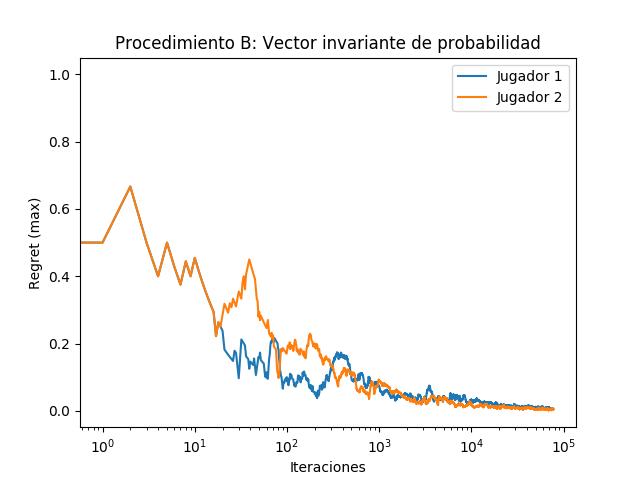
\includegraphics[width=0.4\textwidth]{graficas/coronel-blotto/procedimiento-B.png}
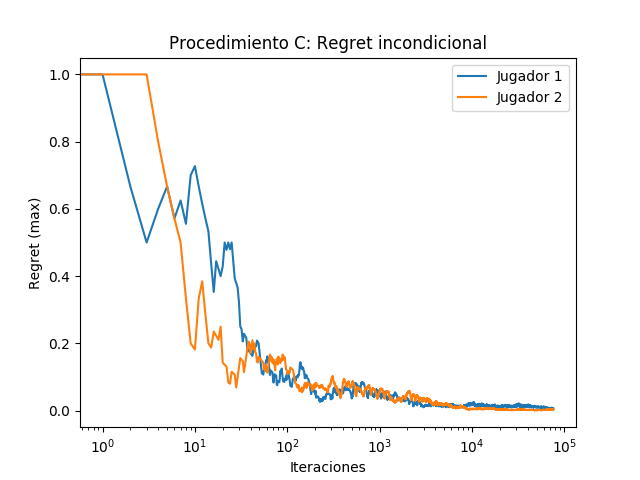
\includegraphics[width=0.4\textwidth]{graficas/coronel-blotto/procedimiento-C.png}
\end{figure}

\newpage